\begin{frame}{Au carrefour de l'histoire des sciences et des humanités numériques}
\begin{figure}
    \centering
    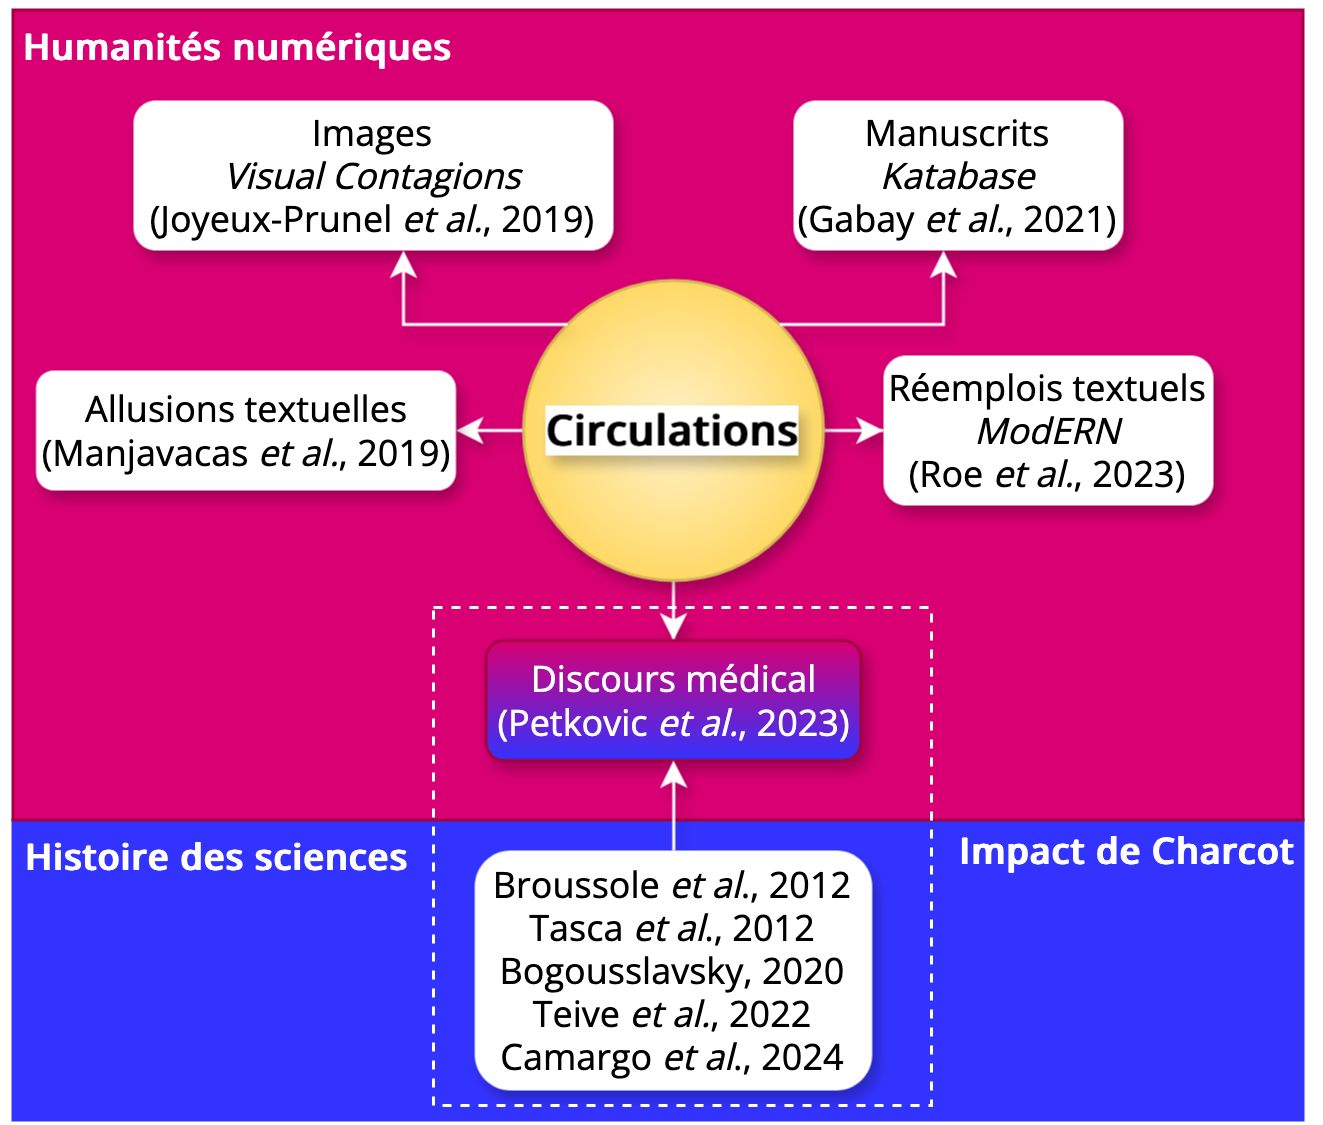
\includegraphics[width=75mm,scale=0.5]{pic/dh_histoire-sciences.png}
    \caption{Études (numériques) des circulations des savoirs.}
    \label{fig:enter-label}
\end{figure}
%\notecite{joyeux2019visual}
%\notecite{gabay2021katabase}
%\notecite{manjavacas2019}
%\notecite{tasca2012women}
%\notecite{bogousslavsky2020}
%\notecite{teive2022thomas}
%\nocite{camargo2024}
%\begin{exampleblock}{}
%\centering
%    \color{deepblue}{\textmd{\textcolor{purple}{Comment pister numériquement la circulation du discours médical de Charcot ?}}}
%\end{exampleblock}
\end{frame}